\section{Transformation composition}

When constructing a scene, an object undergoes multiple transformations, and combining these transformations in a sequence is termed composition.
This typically involves translating and rotating the object in various directions to accurately position it within the scene.
Additionally, achieving rotations around arbitrary axes and scaling with different centers entails combining diverse transformations.
The efficient application of transformation composition is facilitated by the properties of matrix multiplication.

To apply composition, we begin by placing the object's center at position $(p_x, p_y, p_z)$ and orienting its direction at an angle $\alpha$ around the $y$-axis.
Following this initial step, each transformation is performed in order. 
In the case of rotation and translation, it's essential to perform the translation first to avoid complications.

It's noteworthy that, akin to functional programming, matrices appear inside the expression in reverse order concerning the transformations they represent.

\subsection{Transformations around an arbitrary axis}
Now, let's consider the rotation of an object by an angle $\alpha$ about an arbitrary axis passing through the origin.

Suppose we're focusing on a scenario where the direction of the arbitrary axis can be defined using a pair of angles.
Specifically, we can align the $x$-axis with the arbitrary axis by first rotating by an angle $\gamma$ around the $z$-axis, followed by an angle $\beta$ around the $y$-axis.
\begin{figure}[H]
    \centering
    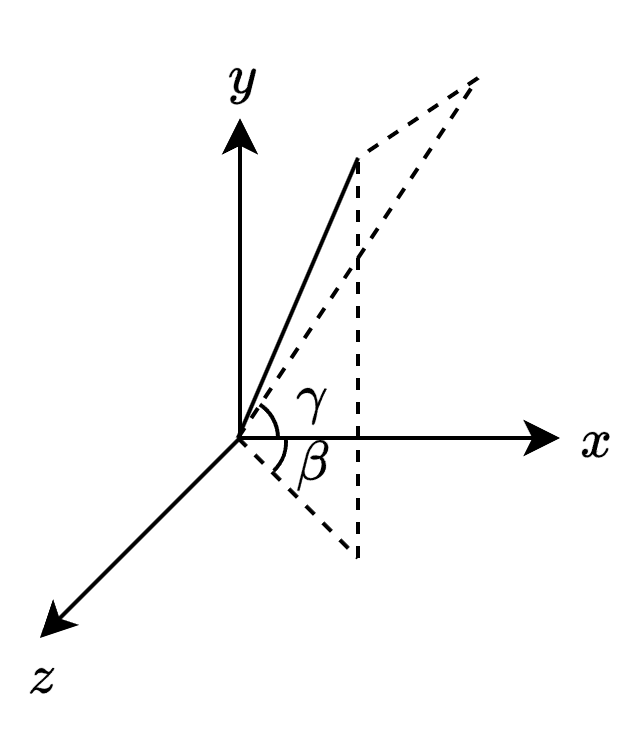
\includegraphics[width=0.25\linewidth]{images/rotationaxis.png}
    \caption{Rotation with an arbitrary axis}
\end{figure}
To position the axis correctly, we need to perform the following transformations: $R^{-1}_y$, $R^{-1}_z$, $R_x$, $R_z$, and $R_y$.

If the axis doesn't pass through the origin but through a point $(p_x,p_y,p_z)$, we must apply a translation $T^{-1}(p_x,p_y,p_z)$ to move it to the origin and then use $T(p_x,p_y,p_z)$ at the end to return the axis to its initial position:
\[R_y{R}_z{R}_x{R}_z^{-1}R_y^{-1}T^{-1}\]
In summary, a rotation of $\alpha$ about an arbitrary axis passing through the point $(p_x,p_y,p_z)$, aligning the $x$-axis by rotating $\gamma$ around the $z$-axis and $\beta$ around the $y$-axis, can be computed as:
\[p^\prime=T(p_x, p_y, p_z) R_y(\beta) R_z(\gamma) R_x(\alpha) R_z{(\gamma)}^{-1} R_y{(\beta)}^{-1} T{(p_x, p_y, p_z)}^{-1} p\]
Similar procedures can be followed for different rotation sequences to align another main axis with the arbitrary one.

These considerations also apply to scaling an object along arbitrary directions and with an arbitrary center. 
They can be extended to generalize shear and perform symmetries about arbitrary planes, axes, or centers.

In many cases, the rotation axis can be represented by a unit vector $n = (n_x, n_y, n_z)$ where $n_x^2 + n_y^2 + n_z^2 = 1$. 
In this scenario, the rotation matrix can be determined using the following pattern:
\[\begin{bmatrix}
    \cos\alpha + n_x^2\left( 1-\cos \alpha \right) & n_x{n}_y\left(1-\cos\alpha\right) -n_z\sin\alpha & n_x{n}_z\left(1-\cos\alpha\right) +n_y\sin\alpha & 0 \\
    n_x{n}_y\left(1-\cos\alpha\right) +n_z\sin\alpha & \cos \alpha + n_y^2\left( 1-\cos\alpha \right) & n_y{n}_z\left(1-\cos\alpha\right) -n_x\sin\alpha & 0 \\
    n_x{n}_z\left(1-\cos\alpha\right) -n_y\sin\alpha & n_y{n}_z\left(1-\cos\alpha\right) +n_x\sin\alpha & \cos\alpha + n_z^2\left( 1-\cos \alpha \right) & 0 \\
    0 & 0 & 0 & 1
\end{bmatrix} \]